\selectlanguage{english}
\clearpage

\section{Test Requirements for IPC Middleware}

This chapter defines the requirements for integration testing in the context of IPC middleware and proposes a structured test strategy. The aim is to address communication-specific challenges such as message loss, timing behavior, and interaction between distributed components. Based on these requirements, a modular and reusable test architecture is designed, serving as the foundation for the implementation and evaluation in later chapters.

\subsection{Analysis of Test Requirements}

Middleware-based systems pose unique testing requirements that differ from classical monolithic systems. Key challenges include the following:

\begin{itemize}
	\item \textbf{Timing behavior:} IPC systems are sensitive to delays, jitter, and message timing. Integration tests must capture whether messages are delivered in time and in correct order.
	
	\item \textbf{Data consistency:} Published data must arrive at all intended subscribers with correct content. Corruption or loss during transmission must be detectable.
	
	\item \textbf{Component coordination:} Integration tests must ensure that multiple processes synchronize correctly. This includes proper startup/shutdown sequences and fault handling.
	
	\item \textbf{Fault Injection:} To evaluate the system’s robustness, integration tests should include controlled fault scenarios. These may involve simulating message loss, injection of delays, disabling specific network routes, or forcing a publisher to stop sending data during transmission. Such tests help verify how well the middleware handles unexpected problems and maintains stable communication.
	
	\item \textbf{Transport abstraction:} Middleware like eCAL supports different transport mechanisms (e.g. TCP, shared memory, UDP). Integration tests should verify that core functionality works across transports.
\end{itemize}


\newpage
\subsection{Functional and Non-Functional Test Objectives}

In the context of IPC middleware, integration testing does not only focus on testing individual components but also on validating how they interact with each other. These interactions include not just message correctness, but also performance, timing, and fault handling. Therefore, integration test objectives are typically divided into two categories: \textit{functional} and \textit{non-functional} requirements~\cite{gorton2006software, tanenbaum2017}.

\subsubsection{Functional Objectives}

Functional objectives ensure that the middleware behaves as expected during normal communication. One important goal is to verify that messages are delivered correctly from publishers to the intended subscribers. This also includes checking topic-based filtering, so that only relevant data is received by each component~\cite{josuttis2007}.
\\
\\
Tests should also cover how the system handles unexpected or incorrect messages. For example, messages with invalid formats, wrong types, or missing fields should not cause the system to crash or behave unpredictably~\cite{burnstein2003practical}.
\\
\\
In addition, if the middleware supports service communication such as Remote Procedure Calls (RPC), tests must confirm that each request gets a correct and timely response. This also includes timeout handling in case a service is not available.

\subsubsection{Non-Functional Objectives}

Non-functional objectives evaluate how well the system performs in different situations. One key metric is \textit{latency}, which measures the time it takes for a message to travel from sender to receiver. Another is \textit{throughput}, which shows how many messages can be transmitted in a given time~\cite{stallings2018}.
\\
\\
Other important aspects include \textit{fault tolerance} and \textit{recovery}. The middleware should be able to handle failures, such as lost network connections or crashed processes, and continue working correctly after a restart~\cite{burns2009real}.
\\
\\
Tests in this category often simulate high message loads, connection losses, or system restarts to see how the middleware reacts and whether it maintains stable communication without data loss.

\subsubsection{Visualization}

To give a clear overview of these requirements, Figure~\ref{fig:mm_requirements} shows a mind map that summarizes the functional and non-functional requirements. This diagram is useful for understanding the full scope of integration testing and serves as a reference for designing test cases.

\begin{figure}[H]
	\centering
	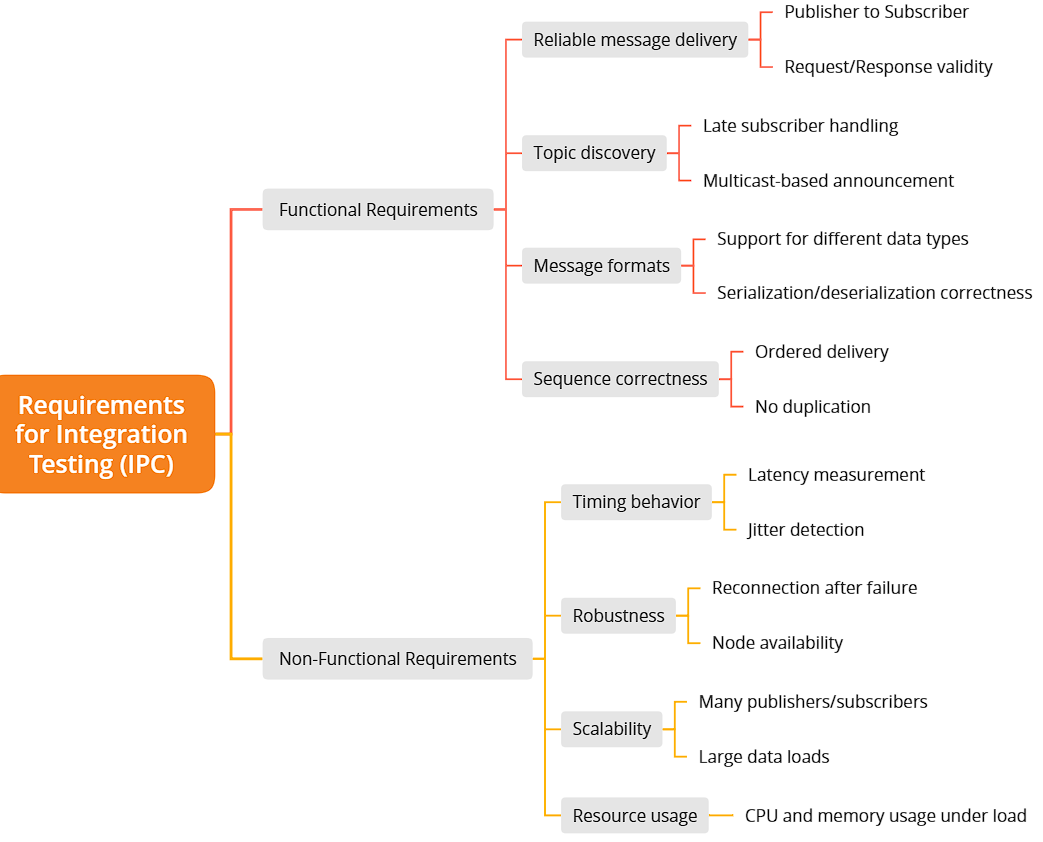
\includegraphics[width=\textwidth]{Images/mm_02_01_requirements.png}
	\caption{Functional, non-functional, and environmental requirements for integration testing of IPC middleware}
	\label{fig:mm_requirements}
\end{figure}

\subsection{Communication Scenarios}

To create meaningful test cases, representative communication scenarios must be modeled. The following scenarios form the foundation for test design:

\begin{itemize}
	\item \textbf{One-to-one communication:} A single publisher sends messages to a single subscriber. Used to test baseline latency and correctness.
	
	\item \textbf{One-to-many communication:} A publisher sends to multiple subscribers. Tests consistency and fan-out behavior.
	
	\item \textbf{Many-to-one communication:} Multiple publishers send to a shared topic. Tests message interleaving and synchronization.
	
	\item \textbf{Multi-host communication:} Tests cross-host communication, IP multicast behavior, and transport compatibility.
	
	\item \textbf{Failure scenarios:} Introduce delays, drop publishers/subscribers mid-test, or overload the system to test resilience.
\end{itemize}

\subsection{Design of a Modular and Reusable Test Strategy}

To address these requirements, a modular test architecture is proposed, consisting of the following layers:

\begin{enumerate}
	\item \textbf{Test scenarios:} Each scenario defines participating nodes, timing, and expected outcomes.
	\item \textbf{Test orchestration:} A framework (e.g., Robot Framework), combined with supporting tools (e.g., Docker), manages the execution flow and the lifecycle of test components.
	\item \textbf{Test Probes:} Lightweight probes are used to monitor the communication process during testing. They capture timestamps, logs, or message payloads for later verification.
	\item \textbf{Result evaluation:} Automated scripts validate logs, output files, or metrics against expected results.
\end{enumerate}

This layered design allows reuse of components across different test cases and enables automation for continuous testing.

\subsection{Summary}

This chapter defined the requirements for integration testing in IPC middleware environments and proposed a test architecture that is both reusable and automation-friendly. These concepts will be implemented and validated using the eCAL framework in the following chapter.


